\section{Overview}

\begin{figure}
  \centering
  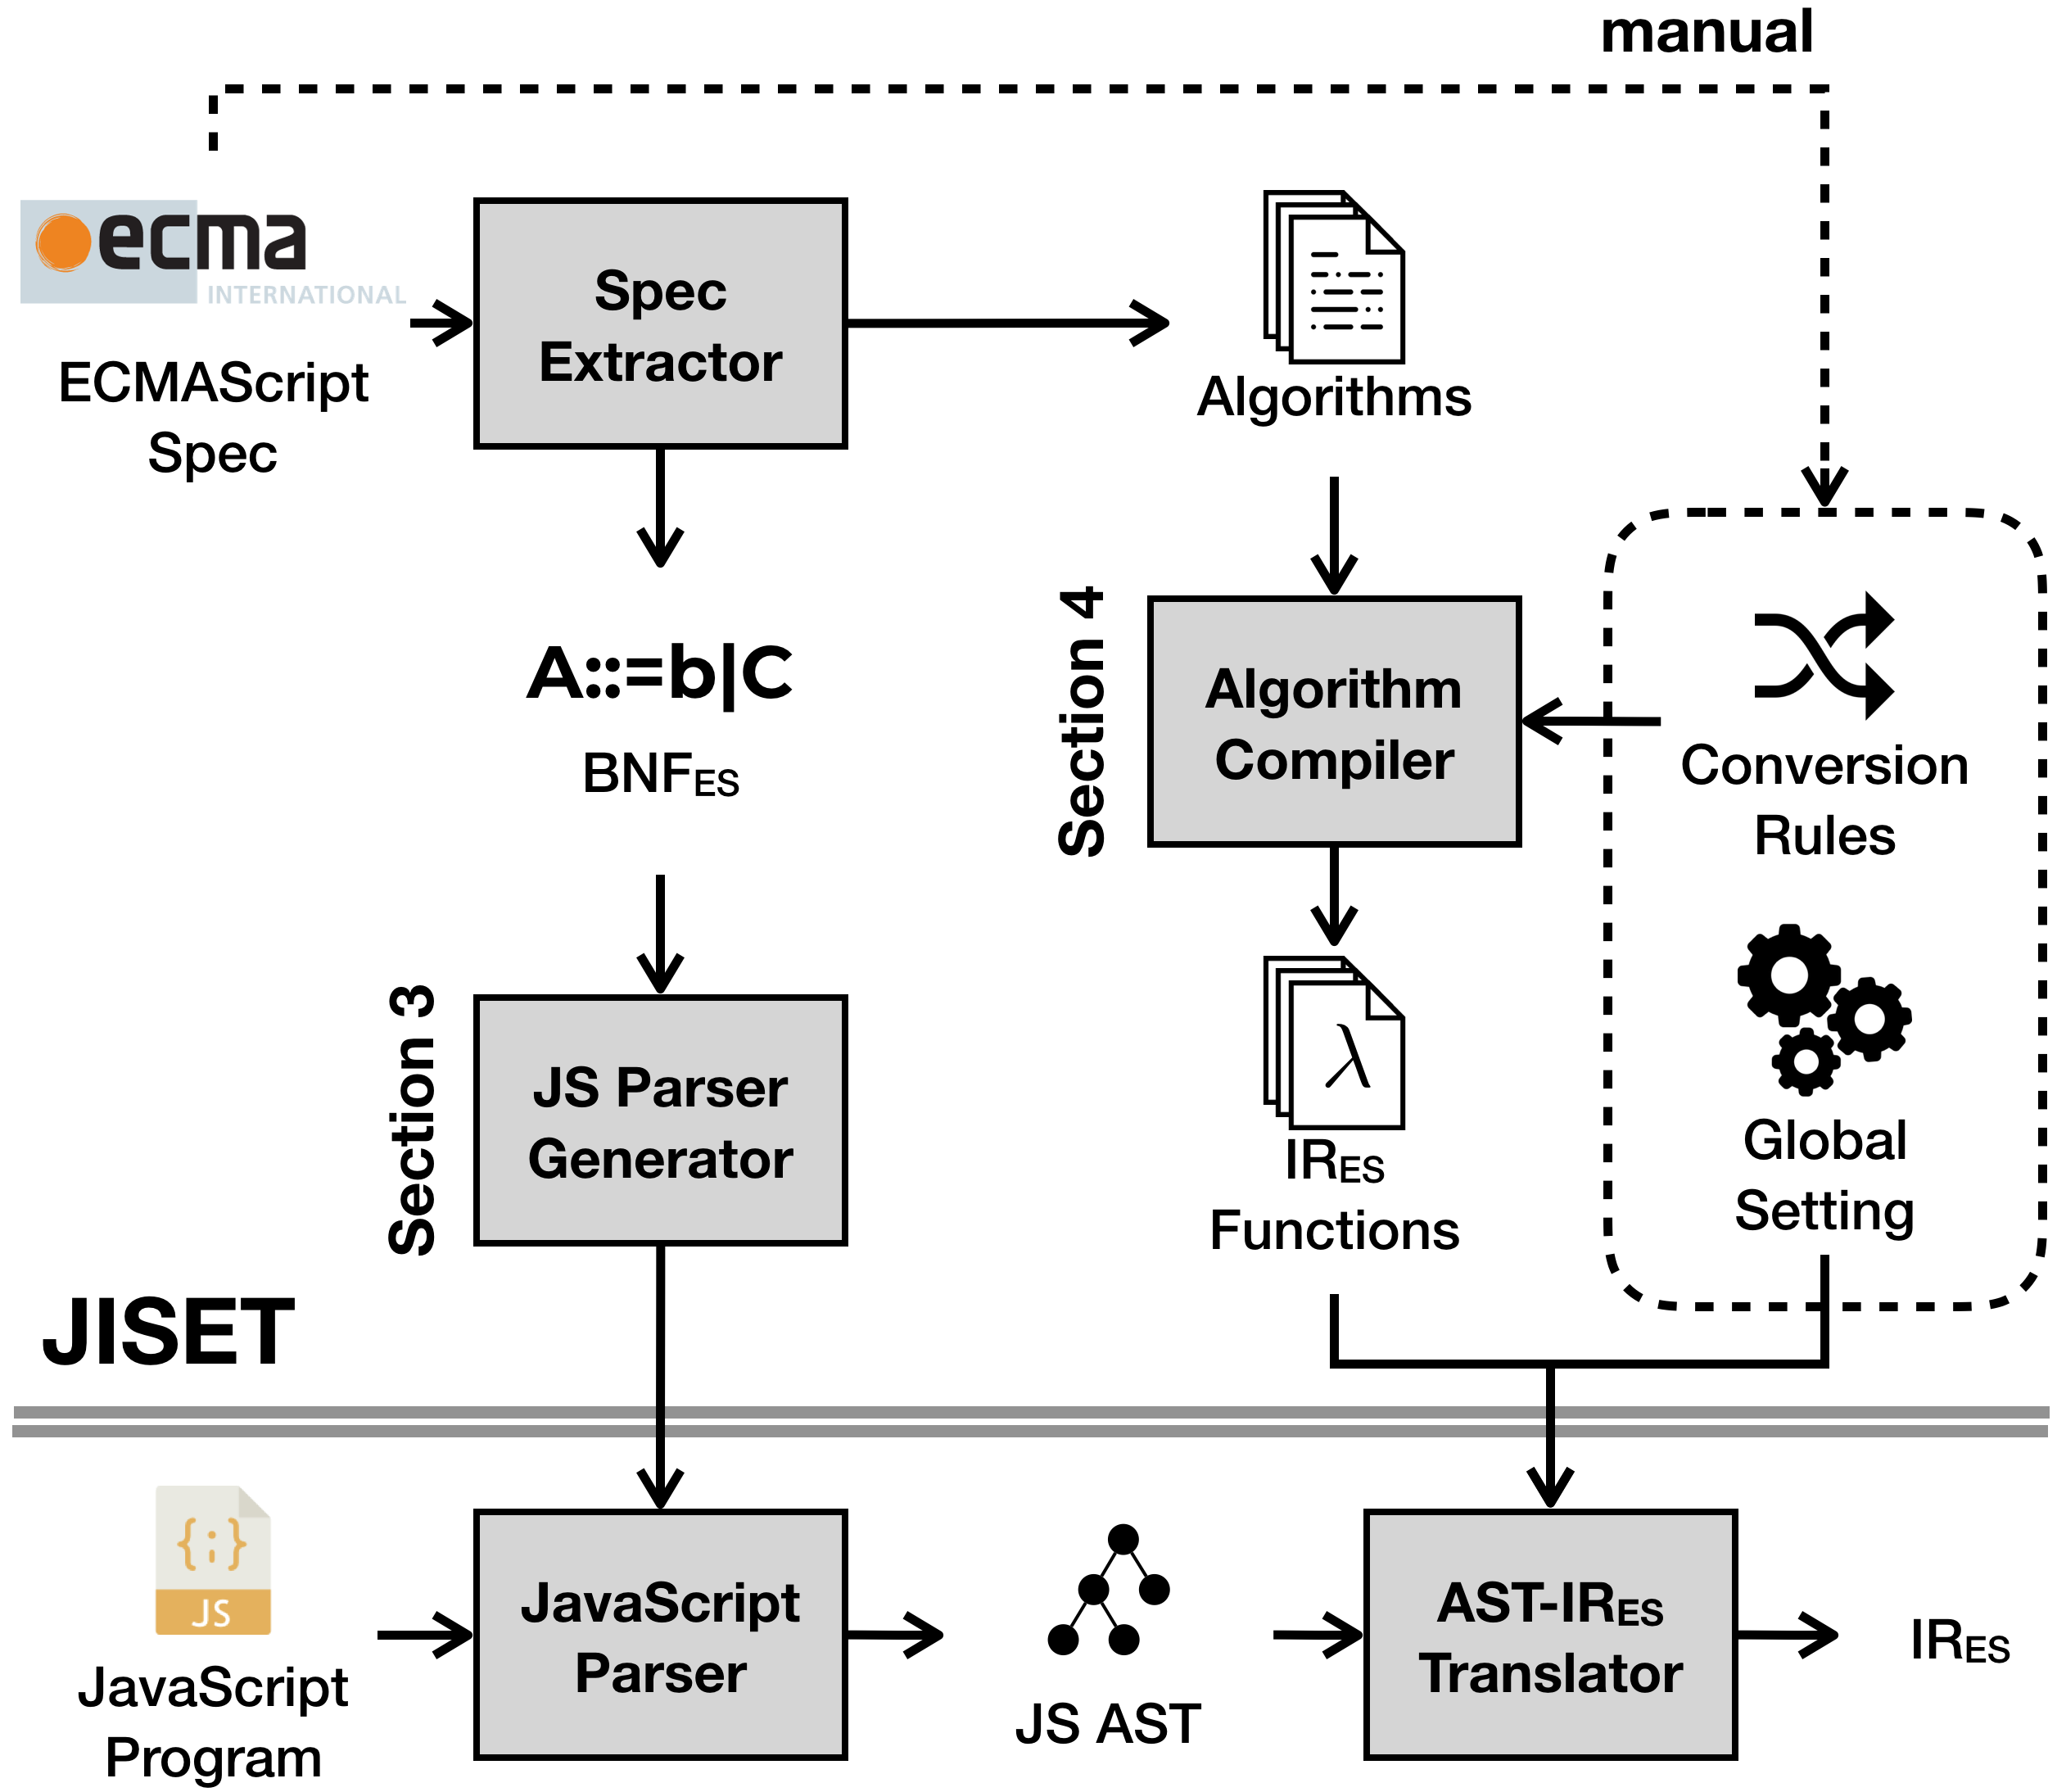
\includegraphics[width=0.5\textwidth]{img/overview.png}
  \caption{Overall structure of JavaScript IR-based Semantics Extraction Toolchain (\( \tool \))}
  \label{fig:overview}
\end{figure}

In this section, we introduce the overall structure of \( \tool \) and the outline of
this paper. The main motivation of automatically extracting syntax and semantics of JavaScript
from ECMAScript specifications is that they are provided as HTML files in well-organized ways.
We utilize such well-organized structures and HTML tag information to extract
syntax and semantics of JavaScript. The overall structure of \( \tool \) is depicted
in Figure~\ref{fig:overview}. For the first step, we develop the spec extractor
in JavaScript to extract syntax and semantics in JSON formats from
the ECMAScript specification HTML file.

\begin{figure}
  \centering
  \begin{subfigure}[t]{0.4\textwidth}
    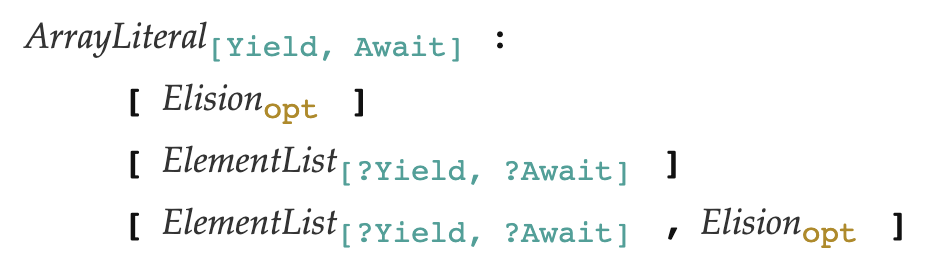
\includegraphics[width=\textwidth]{img/array_literal.png}
    \caption{ArrayLiteral production in ECMAScript 2019 specification.}
    \label{fig:array-literal-es}
  \end{subfigure}
  \begin{subfigure}[t]{0.48\textwidth}
    \begin{lstlisting}[style=myScalastyle]
type P[T] = List[Boolean] => LAParser[T]
lazy val ArrayLiteral: P[ArrayLiteral] = memo {
  case List(Yield, Await) =>
  "[" ~ opt(Elision) ~ "]" ^^ ArrayLiteral0 |
  "[" ~ ElementList(Yield, Await) ~ "]" ^^ ArrayLiteral1 |
  "[" ~ ElementList(Yield, Await) ~ "," ~ opt(Elision) ~ "]" ^^ ArrayLiteral2
}
    \end{lstlisting}
    \caption{The generated parser for ArrayLiteral production.}
    \label{fig:array-literal-parser}
  \end{subfigure}
  \caption{ArrayLiteral grammar production in ECMAScript 2019.}
  \label{fig:array-literal}
\end{figure}

ECMAScript specifications provide their lexical and syntactic grammars in Appendix A
using their own extended Backus-Naur Form (BNF) for ECMAScript.
We call it as \( \bnfes \) and formally define it in Section~\ref{sec:parser}.
The spec extractor to extract grammars written in \( \bnfes \) into JSON files.
For example, Figure~\ref{fig:array-literal-es} denotes the \( ArrayLiteral \) production
in ECMAScript 2020 specification. It takes two boolean parameters
\( Yield \) and \( Await \) and consists of three right-hand sides.
the first right-hand side consists of three symbols; two terminal symbols \( \code{[} \) and
\( \code{]} \), one non-terminal symbol \( Elision_{opt} \). The \( opt \)
subscript denotes that it is optional. In the second and third right-hand sides,
\( ElementList[?Yield, ?Await] \) denotes the parametric non-terminal symbol
with the parameters \( Yield \) and \( Await \) of \( ArrayLiteral \) as two arguments.
The prefix \( ? \) denotes that the given parameter is passed as an argument.

\begin{figure*}[t]
  \centering
  \begin{subfigure}{0.4\textwidth}
    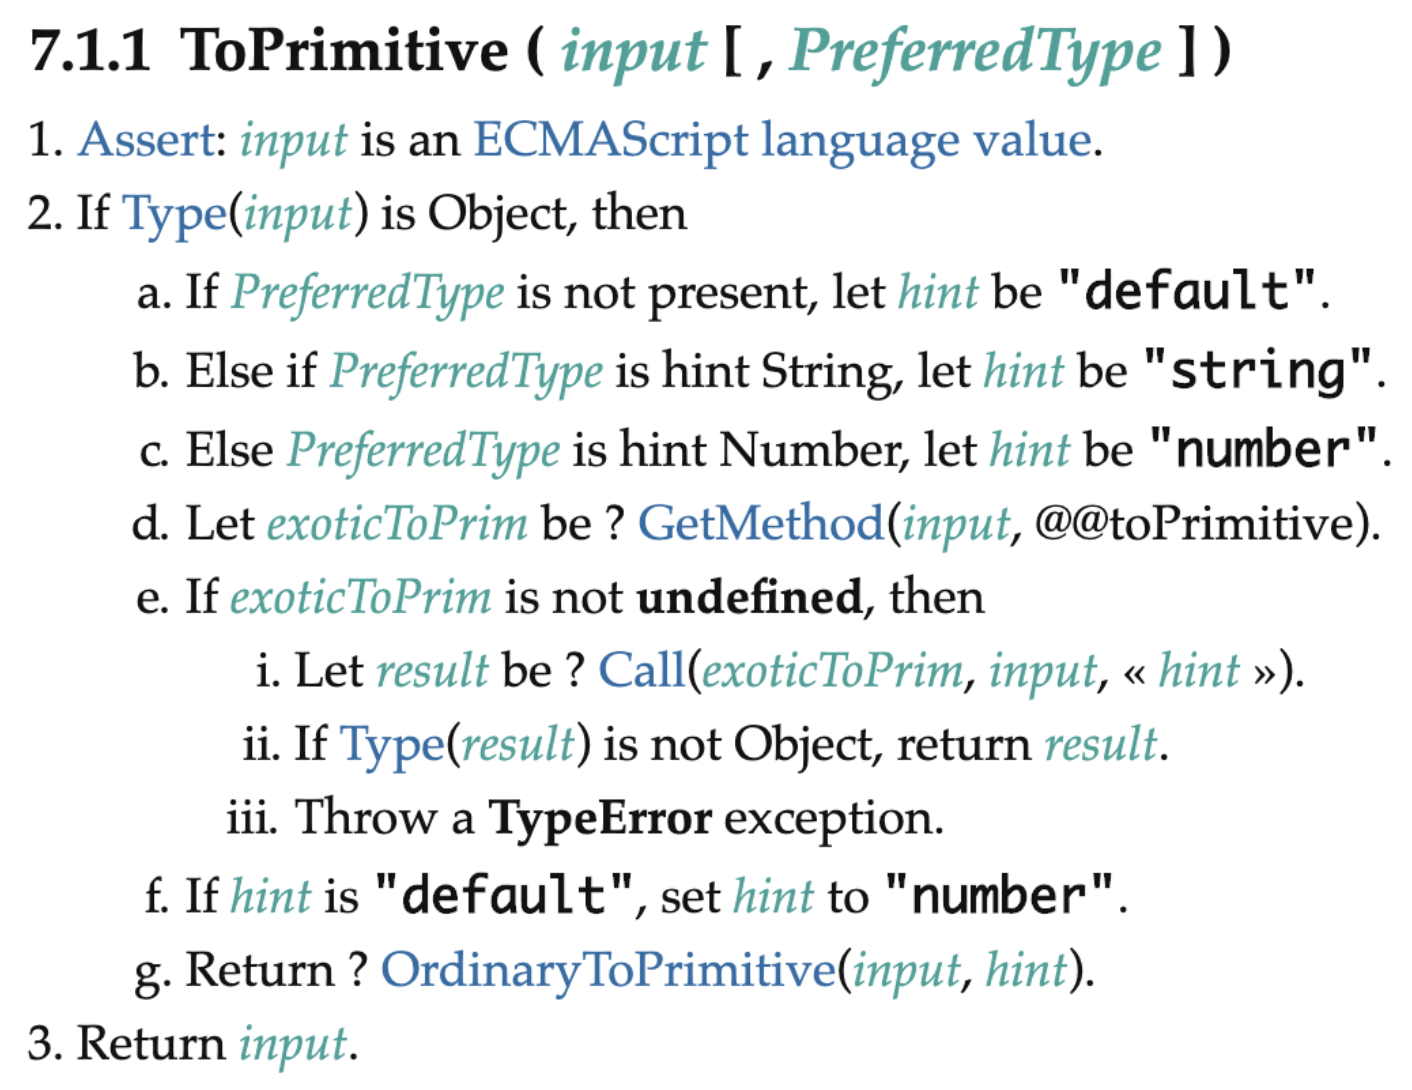
\includegraphics[width=\textwidth]{img/to_primitive.png}
    \subcaption{\( \code{ToPrimitive} \) abstract algorithm in ES2019.}
    \label{fig:to-primitive-es}
  \end{subfigure}
  \qquad
  \begin{subfigure}{0.48\textwidth}
    \begin{lstlisting}[style=ires]
"ToPrimitive" (input, PreferredType) => {
  if (= (Type input) "Object") {
    if (= PreferredType absent) let hint = "default"
    else if (= PreferredType "String") let hint = "string"
    else let hint = "number"
    let exoticToPrim = ? (GetMethod input SYMBOL_toPrimitive)
    if (! (= exoticToPrim undefined)) {
      let result = ? (Call exoticToPrim input (new [hint]))
      if (! (= (Type result) "Object")) return result
      return (Throw INTRINSIC_TypeErrorPrototype)
    }
    if (= hint "default") hint = "number"
    return ? (OrdinaryToPrimitive input hint)
  }
  return input
}
    \end{lstlisting}
    \subcaption{The \( \ires \) funciton for \( \code{ToPrimitive} \)
    abstract algorithm.}
    \label{fig:to-primitive-ires}
  \end{subfigure}
  \caption{\( \code{ToPrimitive} \) abstract algorithms
  and its generated core program.}
  \label{fig:to-primitive}
\end{figure*}

To generate JavaScript parser from the given \( \bnfes \) grammar,
we construct the \textit{parser generator} in Scala.
It synthesizes a JavaScript parser in Scala according to the given \( \bnfes \)
and the generated parser is defined with Scala parser combinators~\cite{scala-parser-combinators}.
Moreover, we propose \textit{lookahead parsers} for correct and fast parsing.
A lookahead parser keeps track of its lookahead, which is the set of
the possible next tokens. With lookahead parsers, the generated parsers are
readable and one-to-one corresponds to each grammar components.
For example, Figure~\ref{fig:array-literal-parser} is the generated parser of
the \( ArrayLiteral \) production in Figure~\ref{fig:array-literal-es}.
Each parser has the \( \code{List[Boolean] => LAParser[T]} \) type because
each production in \( \bnfes \) is parametric with boolean values.
The \( \code{memo} \) is a memoization function for pairs of boolean parameters and result parsers.
for optimizations. The lazy value \( \code{ArrayLiteral} \) corresponds to the \( ArrayLiteral \)
production. In the parser, each String literal such as \( \code{"["} \) or \( \code{"]"} \)
denotes a parser for a terminal symbol. The \( \code{opt} \) helper function creates
optional parsers. The parametric non-terminal \( ElementList \) with arguments \( Yield \)
and \( Await \) is represented as a function call \( \code{ElementList(Yield, Await)} \).
The \( \code{\textasciitilde} \) operator combines two parsers
and the \( \code{\^{}\^{}} \) operator denotes how to construct the abstract syntax trees (AST).
The right side of \( \code{\^{}\^{}} \) is the constructor of AST and each constructor
has the number to denote the order between right-hand sides. For example,
The \( \code{ArrayLiteral0} \) constructor denotes that the first right-hand side of
the \( ArrayLiteral \) production.

The semantics in ECMAScript specifications are described as
abstract algorithms. They are written in structured natural languages
with ordered steps and tagged tokens. The spec extractor extracts each abstract algorithm
with HTML tags because we utilize tag information to discriminate different kinds of tokens.
For example, Figure~\ref{fig:to-primitive-es} is the \( \code{ToPrimitive} \)
abstract algorithm in ECMAScript 2020. It has three steps and
second step consists of seven sub-steps. Each parameter or local variable such as
\( \code{input} \) or \( \code{PreferredType} \) is written with \( \code{<var>} \) HTML tags
and each value is tagged with \( \code{<code>} \).

To extract such abstract algorithms into treatable representations,
we define \( \ires \), a specialized intermediate representation
for ECMAScript abstract algorithms. Then, we develop the \textit{algorithm compiler}
in Scala using also Scala parser combinators to convert given abstract algorithms
into \( \ires \) functions. It is dependent on the conversion rules that consists of two parts;
parsing rules and mapping from each rule into \( \ires \) component.
We explain detailed role of conversion rules in Section~\ref{sec:compiler}.
Thus, each abstract algorithm is converted into a function written in \( \ires \)
through the algorithm compiler. For example, Figure~\ref{fig:to-primitive-ires}
describes the generated \( \ires \) function for the \( \code{ToPrimitive} \)
algorithm. The \( \code{input} \) and \( \code{PreferredType} \) are parameters
of the \( \code{ToPrimitive} \) function. The parameter \( \code{PreferredType} \)
is might be optional but we handle such cases with a special value \( \code{absent} \).
The \( \code{absent} \) value denotes that it is not present.
Thus, the condition of the step 2-a is converted into
the equality check with the \( \code{absent} \).
For the assertions, we omit in this paper but we believe that it could be handled in
the same approach. The specific keywords will be represented as string values.
For instance, the hint Number or the hint String converted into \( \code{"Number"} \)
and \( \code{"String"} \). Moreover, the algorithm compiler modifies prefixes of
symbols from @@ to \( \code{SYMBOL\_} \) and handle exceptions with the corresponding
intrinsic error objects.

Finally, the AST-\( \ires \) translator is constructed with the given \( \ires \)
functions with manually specified global settings. The global settings have
minor but necessary information to evaluate given JavaScript programs.
For example, structure of builtin objects, name aliases for intrinsic objects,
and types of abstract algorithms. Then, we could translate a given JavaScript program
into \( \ires \) through the generated JavaScript parser and AST-\( \ires \) translator
via \( \tool \).

From now, we describe the detailed techniques of \( \tool \).
Section~\ref{sec:parser} formallly defines \( \bnfes \) and how to automatically
generate parsers from given \( \bnfes \) using lookahead parsers.
Section~\ref{sec:compiler} explains abstract algorithms with tagged tokens
and how to compile them into \( \ires \) functions based on
given conversion rules. Moreover, we introduce the rule generation assistant
to easily construct conversion rules. Section~\ref{sec:framework} describes
the implemented details including global settings to evaluate JavaScript programs.
Section~\ref{sec:eval} discusses the effectiveness of \( \tool \) with
four research questions.
Section~\ref{sec:related} discusses related work and Section 8 concludes.
